\chapter{Background}
\section{Stellarium}
Stellarium is a software program designed to enable people to create a virtual planetarium using their home computer \cite{zottistellarium}. It runs on Windows, OSX and Linux/Unix, including Raspberry Pi \cite[p.~6]{zottistellarium}.  Stellarium calculates positions of the Sun, moon, stars and planets based on the time and location defined by the user, and renders them to the display.  Stellarium is used by both amateur and professional astronomers, and is used by the  European Organisation for Astronomical Research in the Southern Hemisphere to facilitate distribution and sharing of visual data among scientists \cite{berglund2008using}. Stellarium has a very high quality graphical display, supporting spherical mirror projection that can be used with a dome \cite{mc2009touring} and is used in many schools and museums because it is both scientifically accurate and visually engaging \cite{berglund2008using}.  Moreover, Stellarium can display constellations from several different cultures and has labels translated to more than 40 languages, making Stellarium both culturally aware and inclusive \cite{berglund2008using}.
For example,  Figures~\ref{fig:WesternCrux} and ~\ref{fig:TukanoTortoise} display the same area of sky, however the first presents the constellations using the western sky lore while the latter presents them in the Tukano sky lore\footnote{The Tukano tribes are indigenous peoples of the northwestern region of Brazil \cite{KnoblochFrancis1976TTIA}.} \cite{reichel1976cosmology}. A comparison reveals that \textit{Scorpius} and \textit{Crux} are referred to as the \textit{Fer-de-lance} and the \textit{Tortoise}. This feature can make Stellarium an extremely useful tool in facilitating multimedia presentations for ethnomusicogy or composing in non-western contexts.

\begin{figure}[htbp]
	\centering
	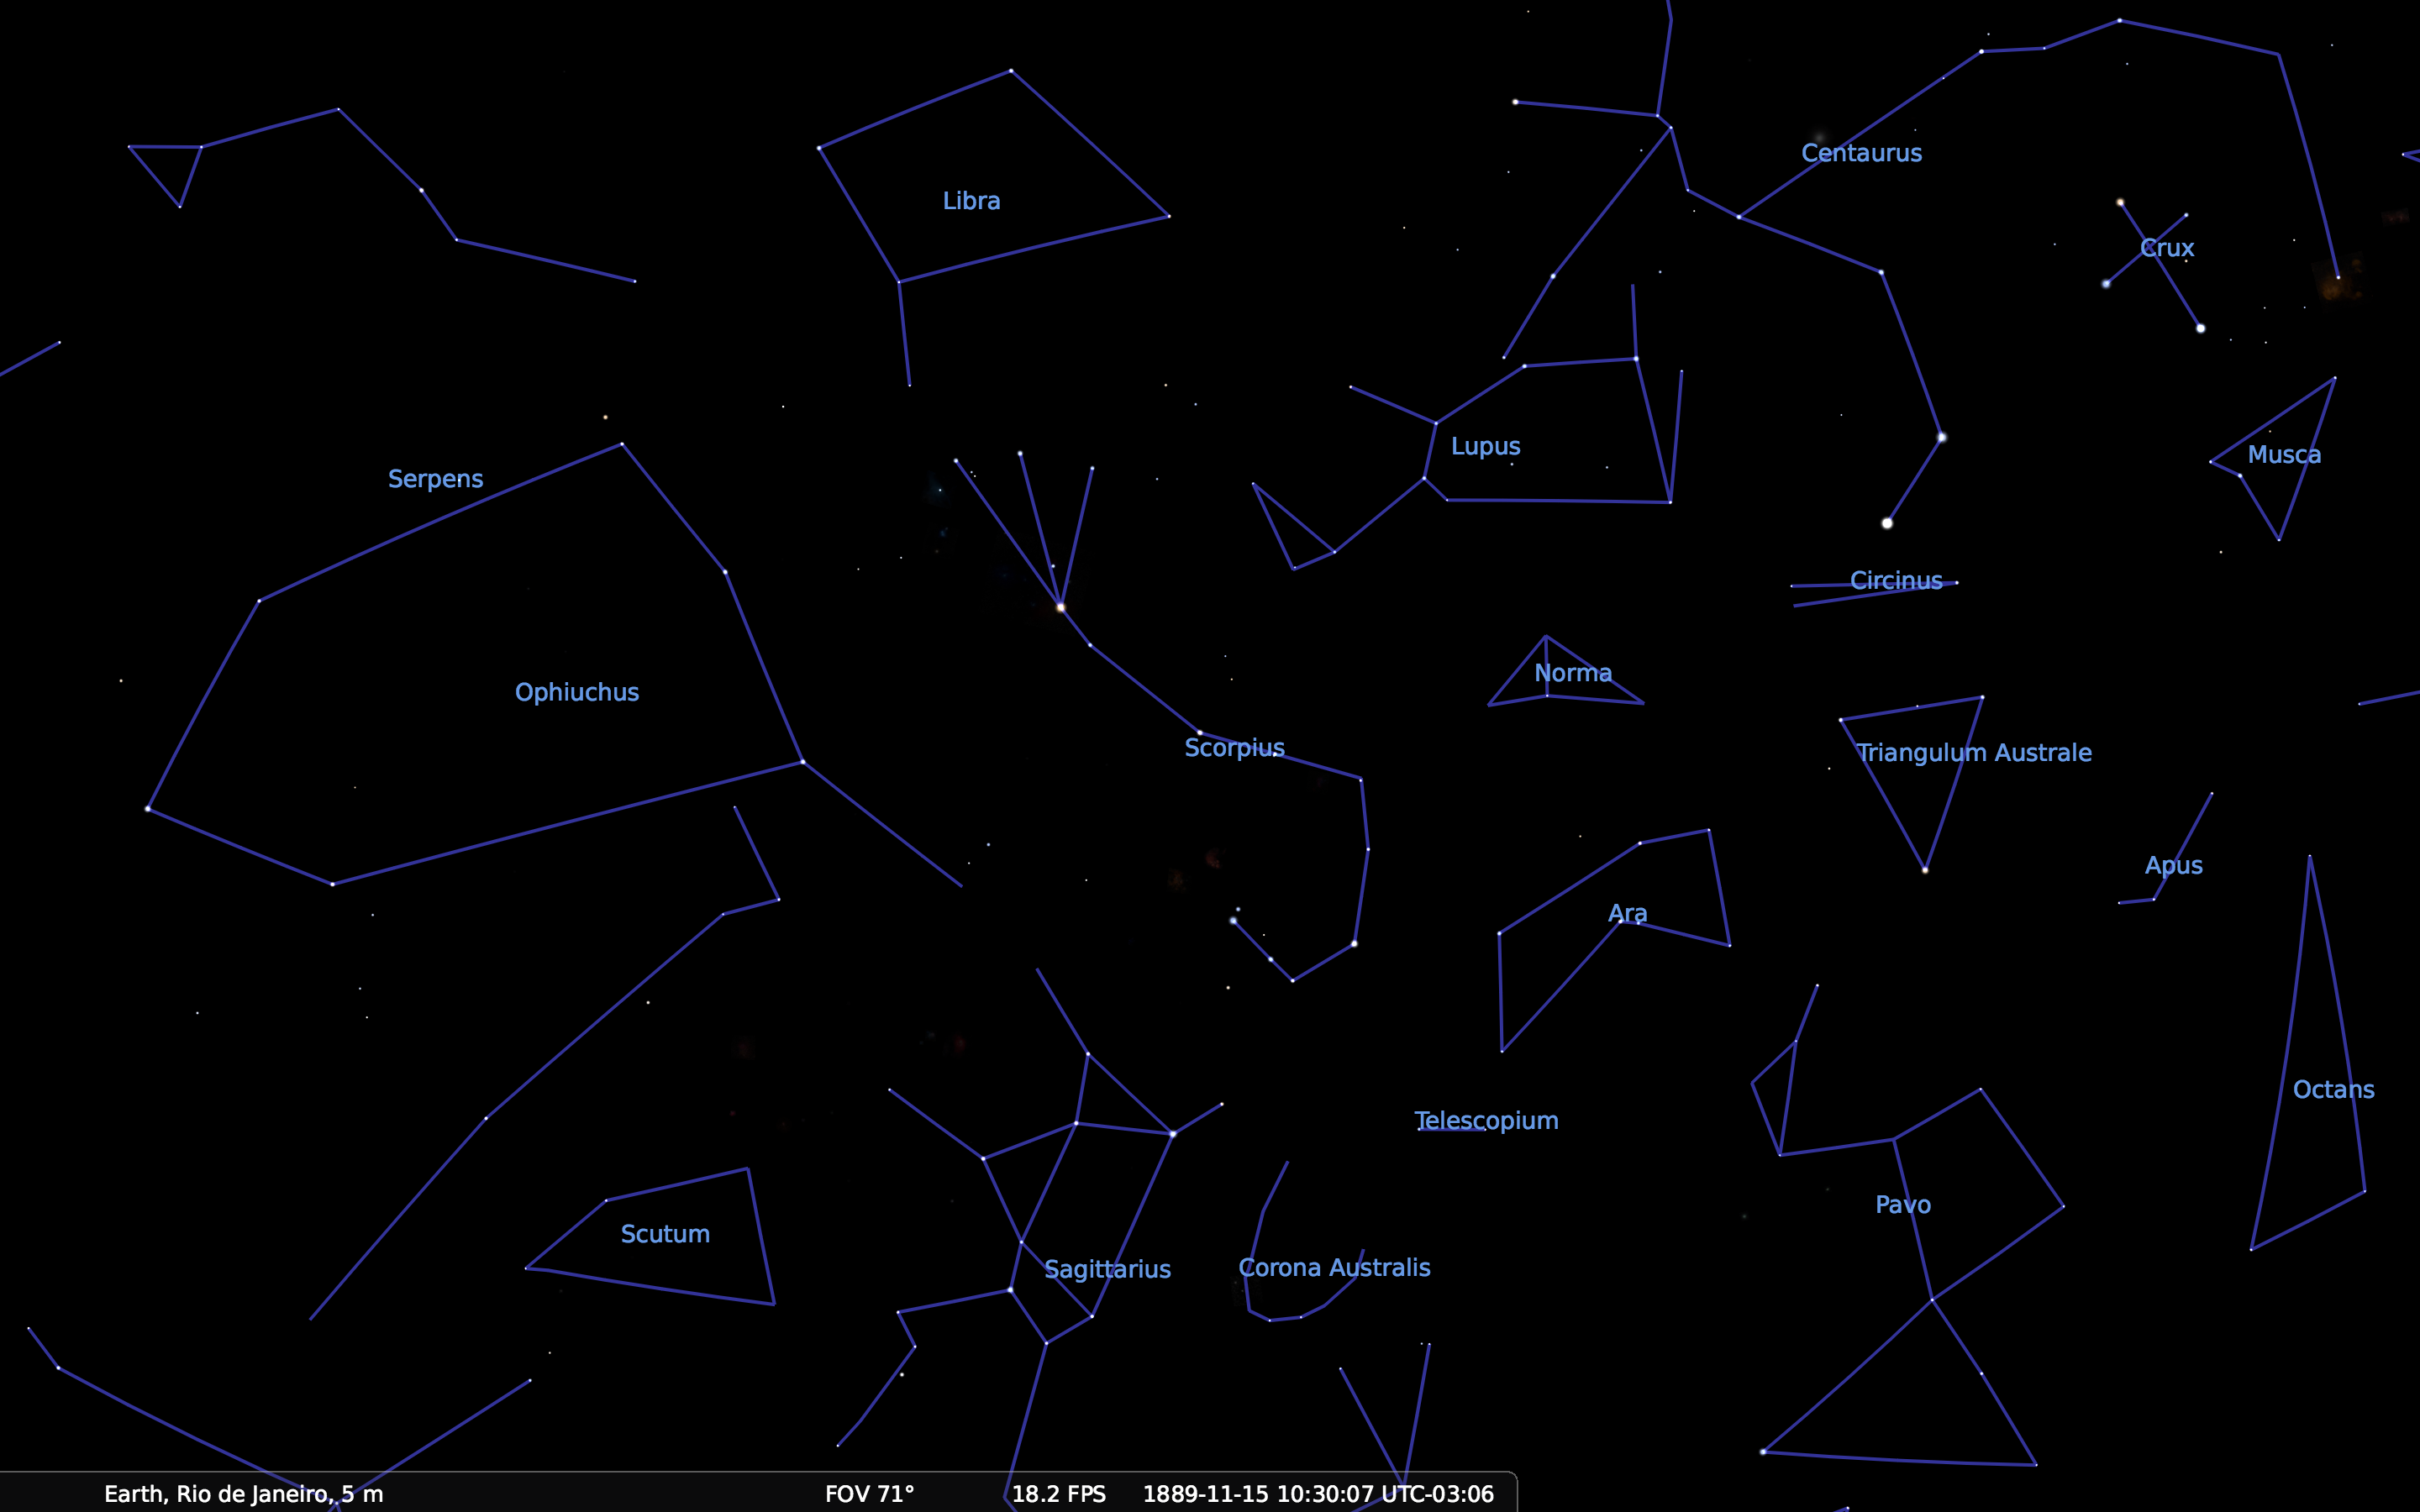
\includegraphics[width=1\columnwidth]{WesternCrux}
	\caption{Constellations displayed in Western sky lore.}
	\label{fig:WesternCrux}
\end{figure}

\begin{figure}[htbp]
	\centering
	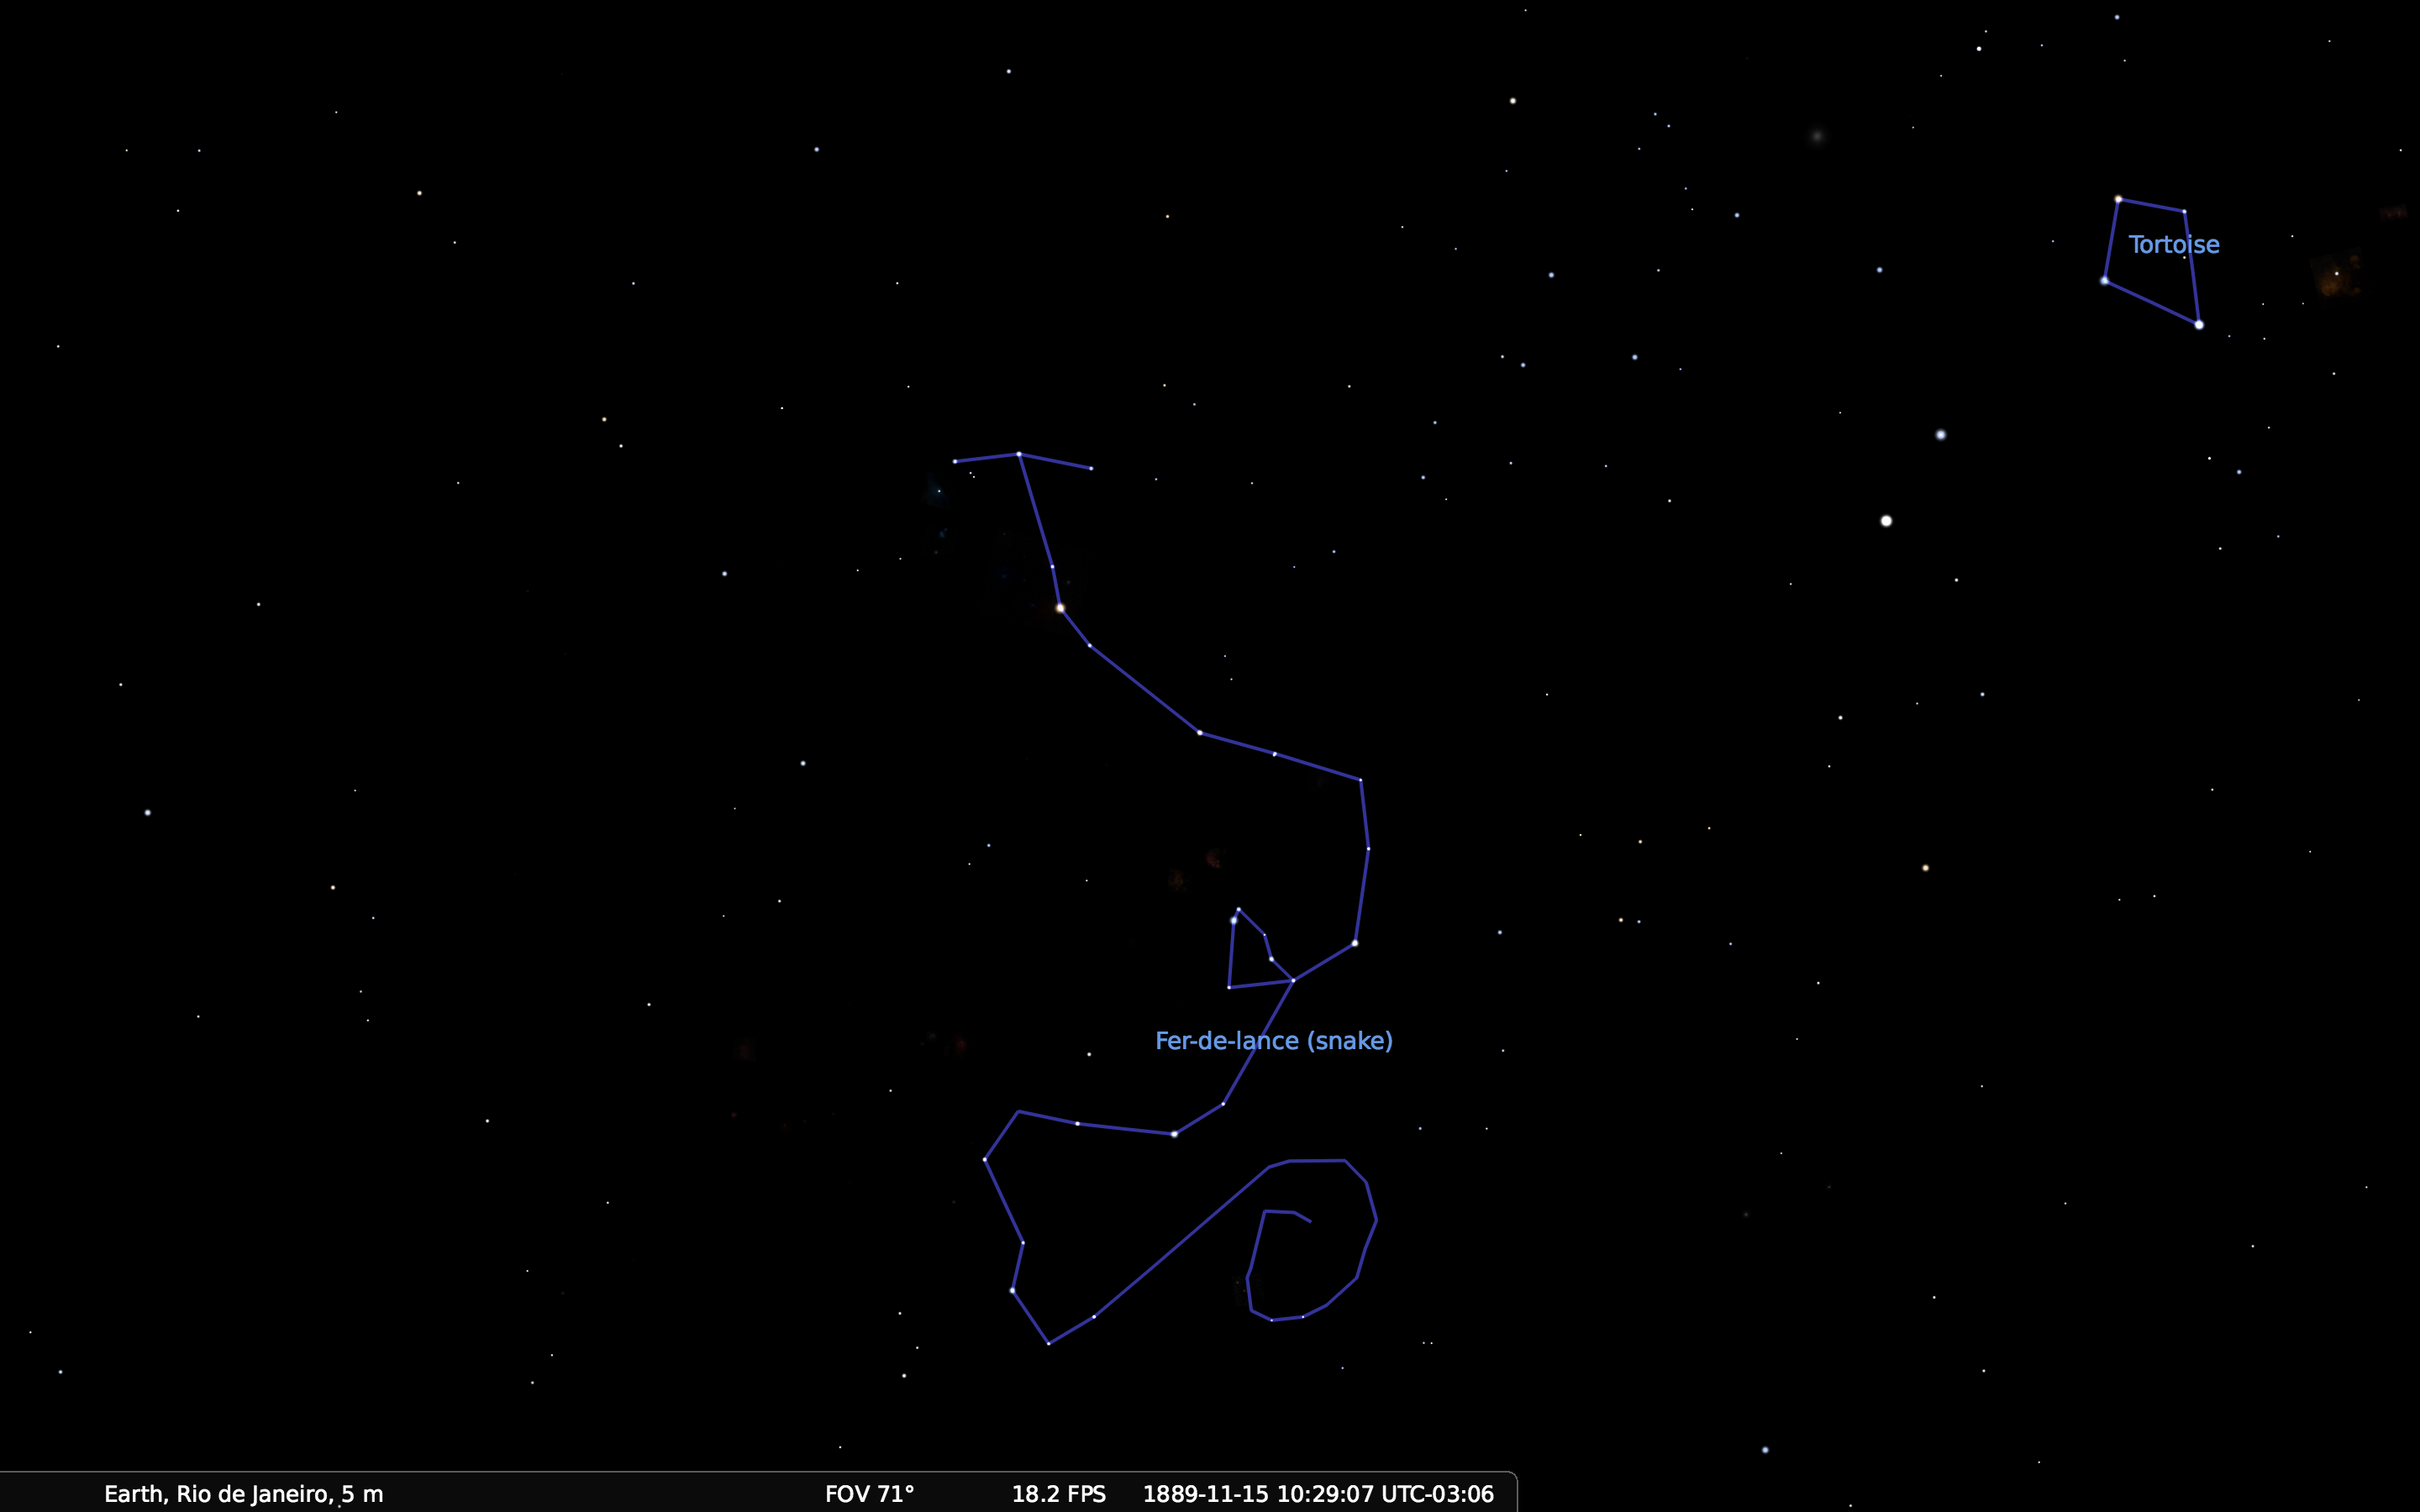
\includegraphics[width=1\columnwidth]{TukanoTortoise}
	\caption{Constellations displayed in Tukano sky lore.}
	\label{fig:TukanoTortoise}
\end{figure}

Many astronomers use Stellarium to display a prediction of the sky for a future time, such as organising a viewing night or planning an astro-photography session \cite{ashley2015computers}. Archaeoastronomers  also use the feature to generate an astronomical display from a location for a period sometime in the past \cite{zotti2014towards}. Also, the landscape feature facilitates a connection between  landscape and  skyscape, so one can map the sky against a landscape for research or aesthetics \cite{zotti2017skyscape}.

Stellarium scripts are written in ECMAScript, also known as Javascript, and enables the programmer to generate and run an automated astronomy presentation, facilitating  automation of all the functionality of Stellarium  \cite{zottistellarium}.

Stellarium has a Remote Control plugin that enables third party programs to communicate with Stellarium via a REST client. This feature was used by the author to create an interactive spacecraft game using a sonic ball as a preliminary test of Stellarium's viability as a responsive performance interface \cite{fraiettaLAC2019}. The plugin also allows clients to query the status of Stellarium, including the area of sky currently being displayed.  The exact celestial vector and field of view displayed are used as the input to the VizieR server in order to obtain data about stars in that location.

\section{VizieR}
VizieR is an online database of high quality astronomical catalogues collected by the Centre de Donn\'ees astronomiques de Strasbourg (CDS), one of whose main goals  ``is to promote the usage of the reliable astronomical catalogues to the astronomical community" \cite[p.~25]{ochsenbein2000vizier}. One of the ways CDS ensures the reliability of their archives and catalogues is to only collect data that has been published or accepted in refereed scientific journals or literature. The number of catalogues available has grown from 3000 in 1999  \cite[p.~24]{ochsenbein2000vizier} to currently 18000 \cite{VizierPage}. Catalogues can be selected by name or based on the wavelength, mission and astronomy type \cite{vizquery}.  Wavelength dictates the frequency spectrum of the data in the catalogue, such as radio, infra-red, optical, x-ray, and Gamma-RAY. The mission indicates the purpose for which the catalogue was created or is used. For example, the purpose of the Kepler Mission is to ``detect Earth-size planets in the habitable zone ... of solar-like stars... , determine their frequency, and identify their characteristics." \cite[p.~2]{koch2010kepler}; and so catalogues created or used within this mission can be specifically targeted. The type of astronomy indicates the subject area of research that the catalogue belongs to; for example,  black holes, galaxy clusters, planetary nebulae, red shifts, and photometry. 

Once a user has selected the database criteria to search, they must provide VizieR  a search window that consists of a target centre and area around that point to search. The target centre is the point on the celestial sphere referenced to a celestial equinox\footnote{The default equinox is J2000 \cite{vizquery}.}, and can be defined by object name,  RA and Dec., or by IAU-coordinates \cite{vizquerytarget}.


\section{Stellar Command Module}
Although it is possible to communicate directly to Stellarium and VizieR directly through the HTTP interface, the stellar position parameters between the two systems are different. Stellarium returns its position information as three dimensional spherical points, with a separate query for the field of view; whereas, VizieR requires the data as a two dimensional geometric point with a defined radius. The Stellar Command module abstracts this information from the client software and removes the requirement to perform these calculations by the client. Stellar Command directs VizieR to query the Hipparcos catalogue because it provides a ``complete all-sky survey of astrometric and photometric parameters for one million stars down to magnitude 11 " \cite [p. ~201]{van1997hipparcos}. An attempt was made using other photometric catalogues, however, it was difficult to obtain consistent results for all sky locations.

The interface required to control both Stellarium and VizieR was HTTP based, so a language that provided network functionality as a fundamental core feature was preferred. Also, it was imperative that third party users of the library should not have to learn a particular programming language, but instead, could easily interface with the library using their preferred music package such as Max MSP, SuperCollider or PD. Furthermore, it would be advantageous for users to be able to integrate the library  into the programming language of their choice, such as C, C++, Python, Ruby, or Java.

Developing the system as a Java Archive (JAR) fulfilled all these requirements. Using a JAR file allowed instantiation from the command line, running as separate processes and using OSC to communicate with other programs. Additionally, many other programming languages can connect directly to a JAR through the Java Native Interface (JNI) \cite{liang1999java}. 
